%
% This document is free; you can redistribute it and/or modify
% it under the terms of the GNU General Public License as published by
% the Free Software Foundation; either version 2 of the License, or
% (at your option) any later version.
%
% This document is distributed in the hope that it will be useful, but
% WITHOUT ANY WARRANTY; without even the implied warranty of
% MERCHANTABILITY or FITNESS FOR A PARTICULAR PURPOSE.  See the GNU
% General Public License for more details.
%
% You should have received a copy of the GNU General Public License
% along with this document; if not, write to the Free Software
% Foundation, Inc., 51 Franklin Street, Fifth Floor, Boston, MA
% 02110-1301, USA.
%
% Author: Bertoli Marco
%
\documentclass[10pt, twoside, a4paper]{book}
\usepackage{fancyhdr}
\usepackage{amsmath,amsfonts,amssymb}
\usepackage{graphicx}
\usepackage[english]{babel}
\usepackage{syntonly}
\usepackage{longtable}
\usepackage{inputenc}
\usepackage{tabularx}
\usepackage{inputenc}
\usepackage{listings}
\usepackage[dvipdfm]{hyperref}
\usepackage{tocbibind}
\hypersetup{ pdftitle={Java Modelling Tools system manual},
pdfauthor={Marco Bertoli}, bookmarksopen=true, bookmarksnumbered,
pdfstartview={FitH}, urlcolor=cyan, citebordercolor=000,
linkbordercolor=000, pdfhighlight=/n, }


% Change default margins
\topmargin -0.5 true in
\setlength{\evensidemargin}{1cm}
\setlength{\hoffset}{-1.5cm}
\setlength{\textwidth}{16.95cm}
\setlength{\textheight}{25cm}
% Space between figure and caption
\setlength{\abovecaptionskip}{-.3cm}

% Define itemize with less margin
\newenvironment{itemize*}
  {\begin{itemize}
    \setlength{\itemsep}{2pt}
    \setlength{\parskip}{0pt}}
  {\end{itemize}}

% Define enumerate with less margin
\newenvironment{enumerate*}
  {\begin{enumerate}
    \setlength{\itemsep}{2pt}
    \setlength{\parskip}{0pt}}
  {\end{enumerate}}

% Define description with less margin
\newenvironment{description*}
  {\begin{description}
    \setlength{\itemsep}{2pt}
    \setlength{\parskip}{0pt}}
  {\end{description}}

\author{Marco Bertoli}

\title{Java Modelling Tools system manual}

\begin{document}
\pagestyle{headings} \pagenumbering{roman} \setcounter{page}{-1}

% Title page
\begin{titlepage}
\begin{figure}[h]
\begin{center}

\includegraphics{img/poli}\\
Performance Evaluation Lab\\
Dipartimento di Elettronica e Informazione\\
Politecnico di Milano - Italy
\end{center}
\end{figure}
\newlength{\centeroffset}
\setlength{\centeroffset}{-0.5\oddsidemargin}
\addtolength{\centeroffset}{0.5\evensidemargin}

 \vspace*{\stretch{1}}
\noindent\hspace*{\centeroffset}\makebox[0pt][l]{\begin{minipage}{\textwidth}
\flushright {\Huge\bfseries Java Modelling Tools}\\
\noindent\rule[-1ex]{9.3cm}{5pt}\\[2.5ex]
\hfill\emph{\Huge system manual}
\end{minipage}}

\vspace{\stretch{0.1}}
\noindent\hspace*{\centeroffset}\makebox[0pt][l]{\begin{minipage}{\textwidth}
\flushright Version~0.1, \today
\end{minipage}}


\vspace{\stretch{2}}


\pagebreak
\begin{small}
  Copyright \copyright 2006 Performance Evaluation Lab - Dipartimento
  di Elettronica e Informazione - Politecnico di Milano.
  All rights reserved.

  Java Modelling Tools is free; you can redistribute it and/or modify it
  under the terms of the GNU General Public License as published by
  the Free Software Foundation; either version 2 of the License, or
  (at your option) any later version.

  Java Modelling Tools is distributed in the hope that it will be useful, but
  WITHOUT ANY WARRANTY; without even the implied warranty of
  MERCHANTABILITY or FITNESS FOR A PARTICULAR PURPOSE\@.  See the GNU
  General Public License for more details.

  You should have received a copy of the GNU General Public License
  along with Java Modelling Tools; if not, write to the Free Software
  Foundation, Inc., 675 Mass Ave, Cambridge, MA 02139, USA.

\end{small}

\end{titlepage}
\cleardoublepage

\tableofcontents \cleardoublepage

\pagenumbering{arabic} \setcounter{page}{1}

% Imports manuals
%
% This document is free; you can redistribute it and/or modify
% it under the terms of the GNU General Public License as published by
% the Free Software Foundation; either version 2 of the License, or
% (at your option) any later version.
%
% This document is distributed in the hope that it will be useful, but
% WITHOUT ANY WARRANTY; without even the implied warranty of
% MERCHANTABILITY or FITNESS FOR A PARTICULAR PURPOSE.  See the GNU
% General Public License for more details.
%
% You should have received a copy of the GNU General Public License
% along with this document; if not, write to the Free Software
% Foundation, Inc., 51 Franklin Street, Fifth Floor, Boston, MA
% 02110-1301, USA.
%
% Author: Bertoli Marco
%
\chapter{Introduction}
This manual is focused on advanced architectural structures of JMT.
It is intended for advanced users that want to interface JMT
computational engines with third party software, or to interact
directly with the XML data layer. More details on the computational
algorithms are also provided.

This manual will not cover any aspect of normal user interaction
with the suite, for such documentation please refer to \emph{JMT
users manual}.

%
% This document is free; you can redistribute it and/or modify
% it under the terms of the GNU General Public License as published by
% the Free Software Foundation; either version 2 of the License, or
% (at your option) any later version.
%
% This document is distributed in the hope that it will be useful, but
% WITHOUT ANY WARRANTY; without even the implied warranty of
% MERCHANTABILITY or FITNESS FOR A PARTICULAR PURPOSE.  See the GNU
% General Public License for more details.
%
% You should have received a copy of the GNU General Public License
% along with this document; if not, write to the Free Software
% Foundation, Inc., 51 Franklin Street, Fifth Floor, Boston, MA
% 02110-1301, USA.
%
% Author: Bertoli Marco
%
\chapter{JMVA}
\label{cha:jmva}
\section{Architecture of the tool}
JMVA has been designed to be very flexible. One important feature is
the complete separation between GUI and computation engine obtained
through an XML layer as shown in \autoref{fig:jmva:Architecture}.
This architecture allows reuse of the analytic engine in other
projects by simply providing a suitable XML input file (see
\autoref{sec:jmva:XML} for details).

\begin{figure}[htbp]
    \begin{center}
        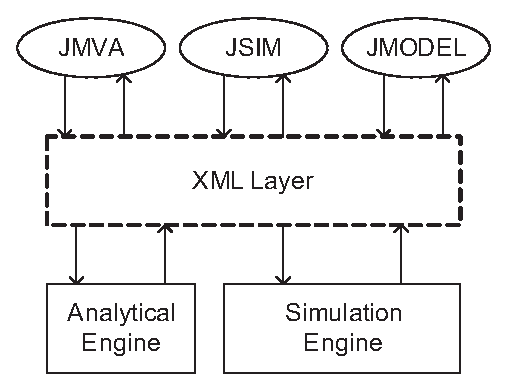
\includegraphics[scale=.65]{img/jmva/Architecture}
    \end{center}
    \caption{JMT Architecture}
    \label{fig:jmva:Architecture}
\end{figure}

Model solution with analytical engine can be started by executing
the \textbf{solve(File XMLFile)} method of the
\textbf{jmt.gui.exact.link.SolverDispatcher} class. The
\texttt{XMLFile} parameter is a well formed XML File according to
\emph{JMTmodel.xsd} schema described in \autoref{sec:jmva:XML}. At
the end of the computation, performance indices will be placed into
the \textbf{solutions} element of input file.

\section{XML format}
\label{sec:jmva:XML}
% Highlight java code
\lstset{language=XML,usekeywordsintag=true, basicstyle=\small} JMVA
XML format is simple and can be written even by hands. The syntax of
that file is specified in \emph{JMTModel.xsd} and is graphically
represented in \autoref{fig:jmva:stylesheet}.

\begin{figure}[p]
    \begin{center}
        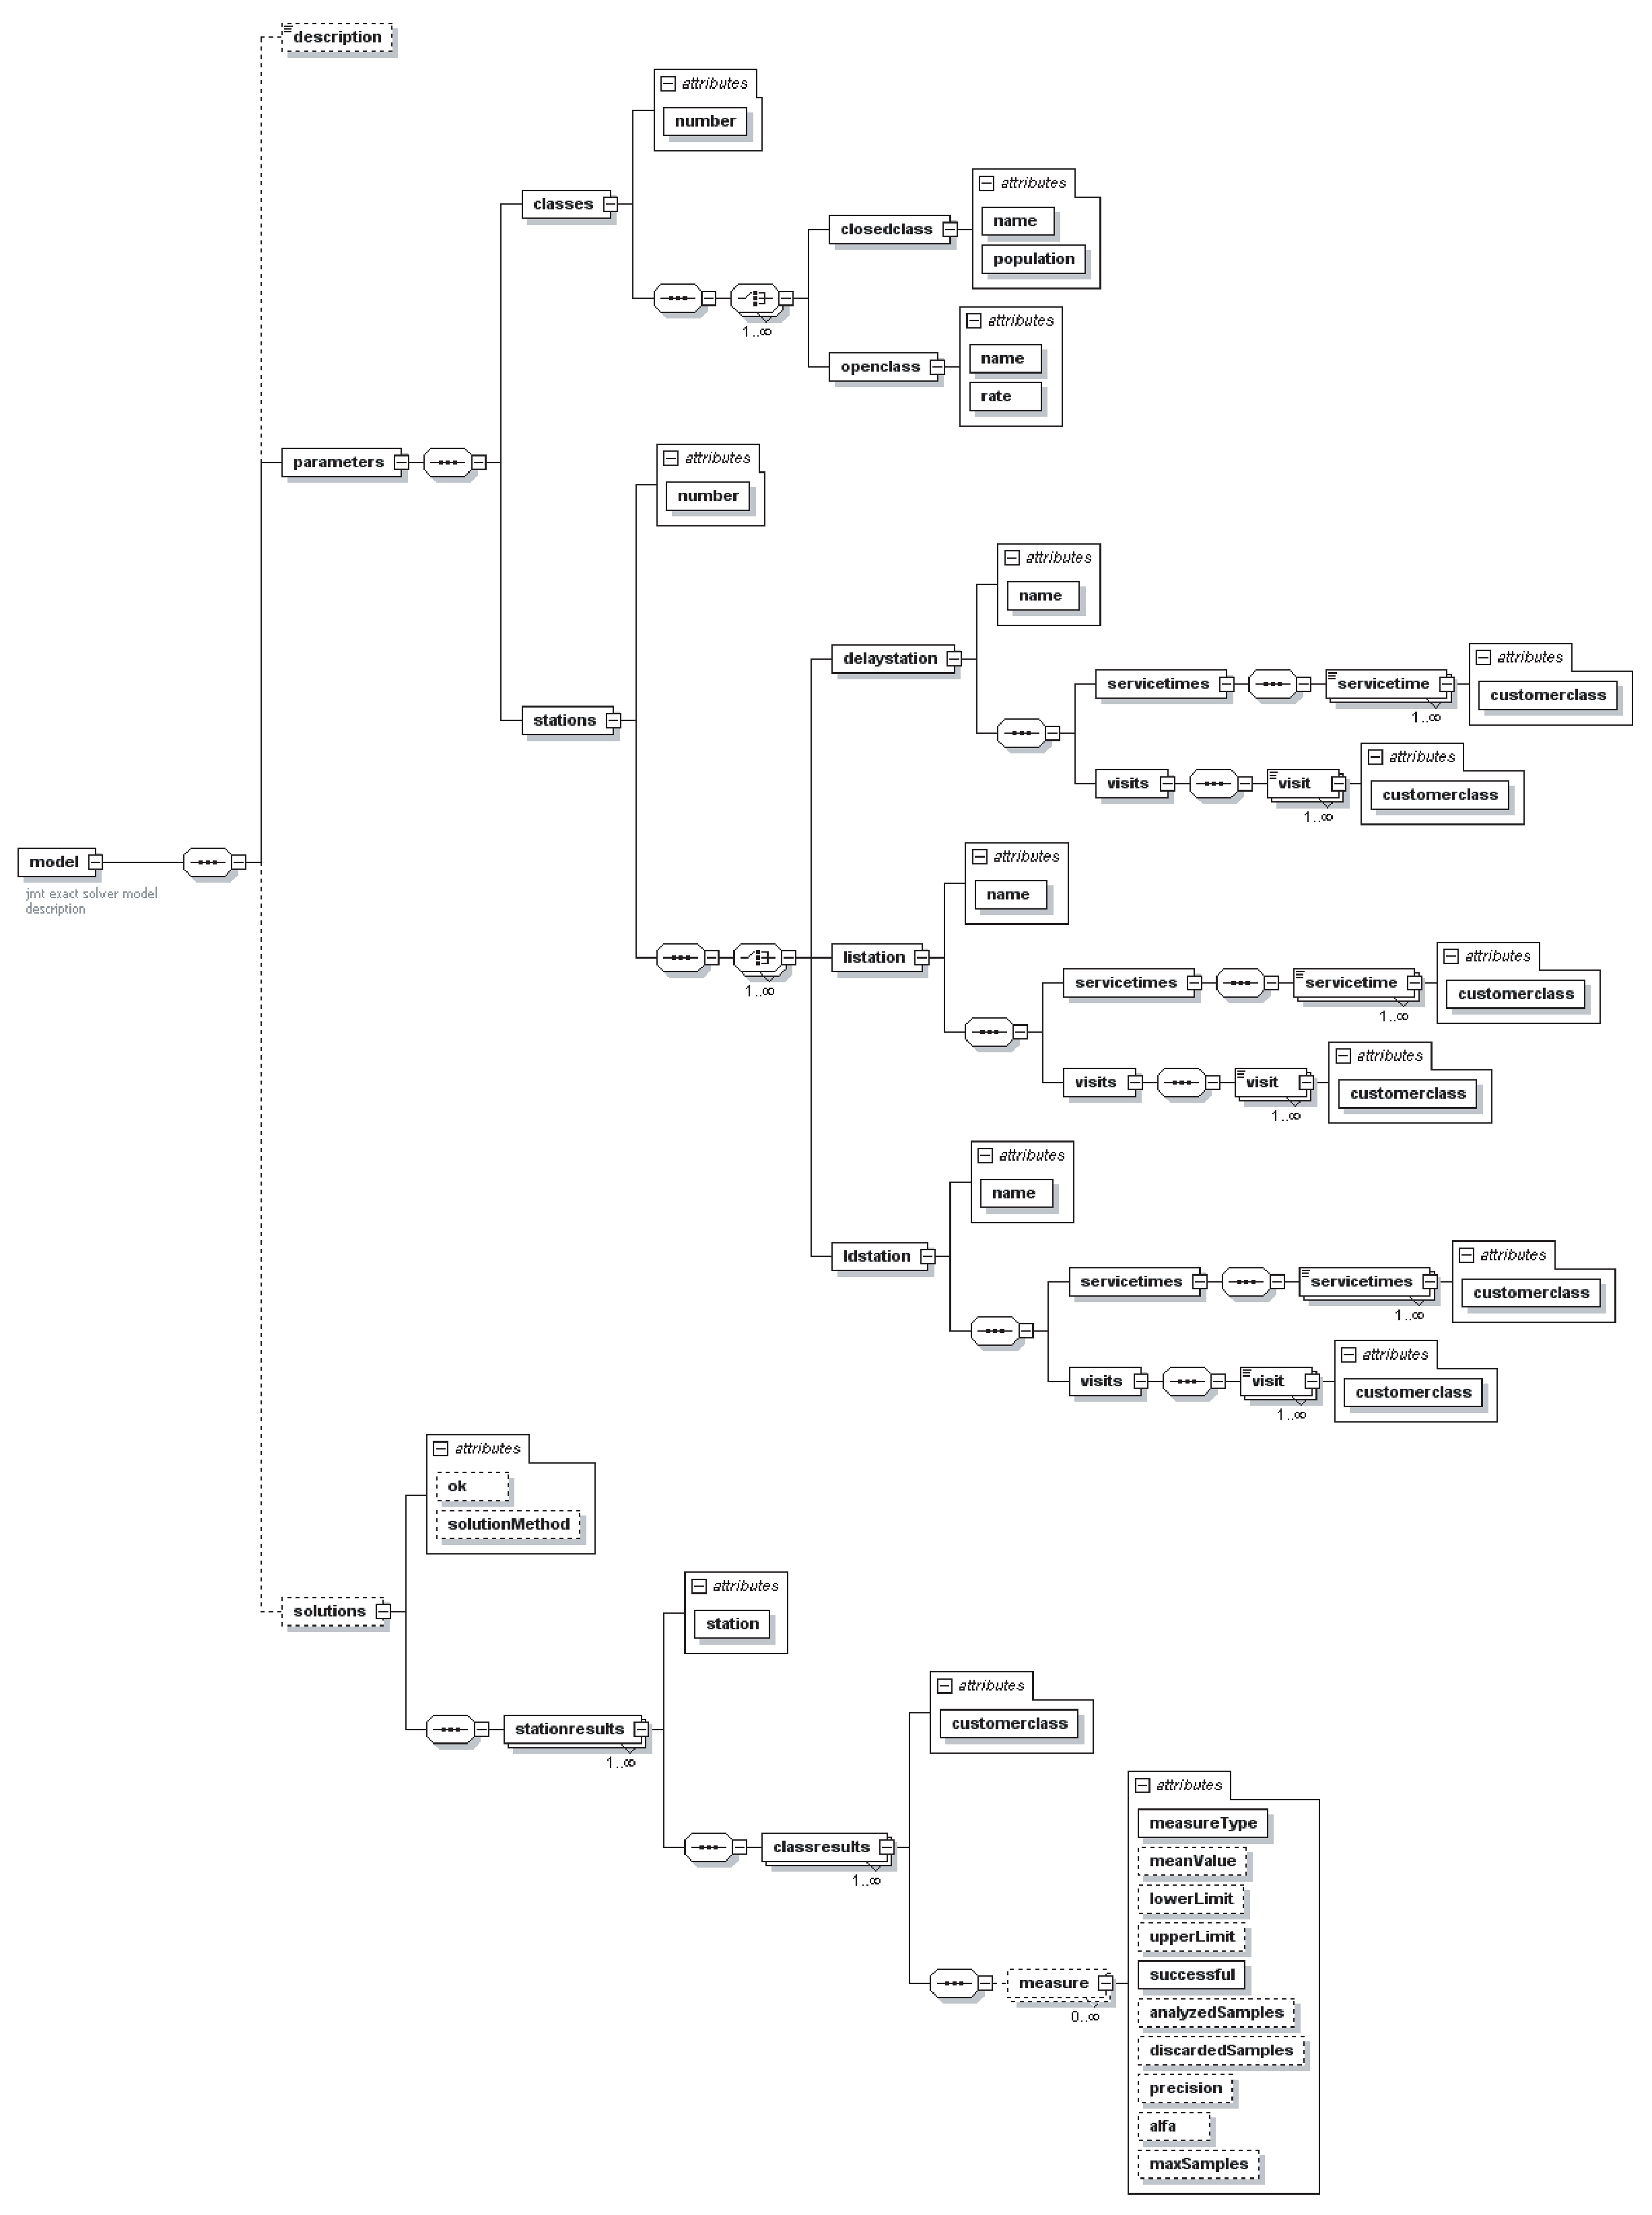
\includegraphics[width=1\textwidth]{img/jmva/JMTmodel}
    \end{center}
    \caption{JMTModel.xsd stylesheet graphic representation}
    \label{fig:jmva:stylesheet}
\end{figure}

The root element is \textbf{model} and can include an optional
\textbf{description} of the model, a section with \textbf{solutions}
(that is parameterized by the solver engine) and the section
\textbf{parameters} used to specify the network to be solved.

The section \textbf{parameters} contains the section
\textbf{classes} that has for attribute the global \textbf{number}
of classes and can include from one to infinite \textbf{openclass}
or \textbf{closedclass}. \textbf{openclass} must specify a
\textbf{name} and arrival \textbf{rate}, while \textbf{closedclass}
must specify a \textbf{name} and \textbf{population}.

For example to define one closed class with $N = 10$ and one open
class with $\lambda = 0.5$ the code will be:

\begin{lstlisting}[gobble=7]
        <classes number="2">
            <closedclass name="ClosedClass" population="10"/>
            <openclass name="OpenClass" rate="0.5"/>
        </classes>
\end{lstlisting}

The other section of \textbf{parameters} is \textbf{stations}. This
element has \textbf{number} as attribute (like classes) and is
composed from one to infinite elements of the following types:
\begin{description*}
    \item[delaystation] is a delay station (infinite server)
    \item[listation] is a load independent station
    \item[ldstation] is a load dependent station
\end{description*}
All the elements are defined with the same procedure. For each
station the \textbf{name} attribute should be specified and two
elements named \textbf{servicetimes} and \textbf{visits} must be
included. \textbf{servicetimes} must include a list of at least one
\textbf{servicetime} element and \textbf{visits} must include a list
of at least one \textbf{visit} element. Both \textbf{visit} and
\textbf{servicetime} elements have a \texttt{double} numeric value
and each element has an attribute named \textbf{customerclass} that
is used to associate a value of service time/visit with the
corresponding customer class.

The only exception is \textbf{servicetime} parameter for a load
dependent station. In this case the value is not a double but is a
list of \texttt{double} separated by the special character
\textbf{;} . The list is ordered for ascending values of number of
jobs in the station, starting from 1 to number of customer $N$ of
the closed class of the model.

For example in a model with one closed class, named \emph{Class1},
with $N=5$ and three stations: a load independent with service
demand 1, a delay with service demand 2 and a load dependent with
$D(N)=N+2$, the following code should be used for the station
definition:

\begin{lstlisting}[gobble=7]
        <stations number="3">
            <listation name="LoadIndependent">
                <servicetimes>
                    <servicetime customerclass="Class1">
                        1.0</servicetime>
                </servicetimes>
                <visits>
                    <visit customerclass="Class1">1.0</visit>
                </visits>
            </listation>
            <delaystation name="Delay">
                <servicetimes>
                    <servicetime customerclass="Class1">
                        2.0</servicetime>
                </servicetimes>
                <visits>
                    <visit customerclass="Class1">1.0</visit>
                </visits>
            </delaystation>
            <ldstation name="LoadDependent">
                <servicetimes>
                    <servicetimes customerclass="Class1">
                        3.0;4.0;5.0;6.0;7.0</servicetimes>
                </servicetimes>
                <visits>
                    <visit customerclass="Class1">1.0</visit>
                </visits>
            </ldstation>
        </stations>
\end{lstlisting}

Also the computed performance indices are stored in the same XML
document. \textbf{solutions} has two attributes: \textbf{ok} that
indicates if the computation was successful and
\textbf{solutionMethod} that indicates if solution was obtained
through analytical engine or simulator. Inside a \textbf{solutions}
element there is a list of one or more \textbf{stationresults}, an
element with station \textbf{name} as its attribute that contains
one or more \textbf{classresults}, an element with class name
(\textbf{customerclass}) as its attribute. This peculiar structure
is needed to store a matrix of results. Each \textbf{classresults}
element contains any number of \textbf{measure} elements that are
used to store computed performance indices. \textbf{measure} has the
following attributes:
\begin{description}
\item[measureType] type of performance index, can be one between \emph{Queue
length}, \emph{Throughput}, \emph{Residence time} and
\emph{Utilization}
\item[successful] boolean field that indicates if measure was
computed correctly
\item[meanValue] (optional) computed value. This field is optional
and will be always present if successful=true
\item[lowerLimit] (optional) lower limit of confidence interval. As
MVA produces \emph{exact} solution, this field is used only when
model is solved with simulator
\item[upperLimit] (optional) upper limit of confidence interval. As
MVA produces \emph{exact} solution, this field is used only when
model is solved with simulator
\item[analyzedSamples] (optional) number of samples analyzed by the
simulator
\item[discardedSamples] (optional) number of samples discarded by the
simulator
\item[precision] (optional) maximum relative error allowed by
simulator
\item[alfa] (optional) confidence interval required to simulator
\item[maxSamples] (optional) maximum number of samples allowed by
simulator
\end{description}
Note that only the first three elements of the above description
will be saved by JMVA. The others are used when the model is solved
using the simulator JSIM. For example, a model with one class (named
\emph{Class1}) and two stations (named \emph{Station1} and
\emph{Station2}) will produce the following solutions:
\begin{lstlisting}[gobble=3]
    <solutions ok="true" solutionMethod="analytical">
        <stationresults station="Station1">
            <classresults customerclass="Class1">
                <measure meanValue="9.930828575679609"
                    measureType="Queue length"
                    successful="true"/>
                <measure meanValue="5.467534818643117"
                    measureType="Throughput"
                    successful="true"/>
                <measure meanValue="1.8163265356477696"
                   measureType="Residence time"
                   successful="true"/>
                <measure meanValue="0.9999999999987986"
                    measureType="Utilization"
                    successful="true"/>
            </classresults>
        </stationresults>
        <stationresults station="Station2">
            <classresults customerclass="Class1">
                <measure meanValue="0.06917142432039082"
                    measureType="Queue length"
                    successful="true"/>
                <measure meanValue="5.467534818643117"
                    measureType="Throughput"
                    successful="true"/>
                <measure meanValue="0.01265130019557098"
                    measureType="Residence time"
                    successful="true"/>
                <measure meanValue="0.06469628980696993"
                    measureType="Utilization"
                    successful="true"/>
            </classresults>
        </stationresults>
    </solutions>
\end{lstlisting}

It is important to point out that JMVA stores and loads model and
results in \emph{exactly} the same XML format used to dialogue with
the analytical engine. The best practice to learn rapidly its syntax
is to create a model using JMVA GUI, store it in any place and open
it with a text editor.

%%
% This document is free; you can redistribute it and/or modify
% it under the terms of the GNU General Public License as published by
% the Free Software Foundation; either version 2 of the License, or
% (at your option) any later version.
%
% This document is distributed in the hope that it will be useful, but
% WITHOUT ANY WARRANTY; without even the implied warranty of
% MERCHANTABILITY or FITNESS FOR A PARTICULAR PURPOSE.  See the GNU
% General Public License for more details.
%
% You should have received a copy of the GNU General Public License
% along with this document; if not, write to the Free Software
% Foundation, Inc., 51 Franklin Street, Fifth Floor, Boston, MA
% 02110-1301, USA.
%
% Author: Bertoli Marco
%
\chapter{JSIM}
\label{cha:jsim}
\section{Simulation engine architecture}
\subsection{General architecture}
All simulator engine classes are included in \texttt{jmt.engine}
package: its structure is shown in \autoref{fig:jsim:package}.

\begin{figure}[htbp]
    \begin{center}
        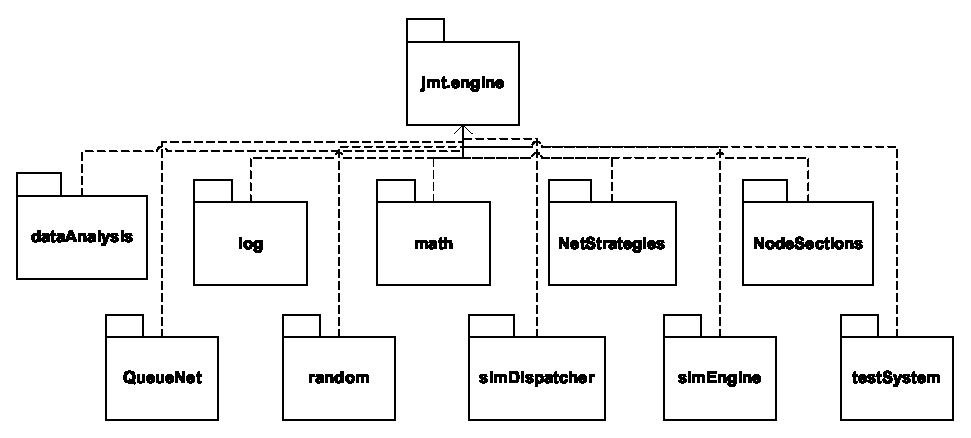
\includegraphics[scale=.65]{img/jsim/Package_engine}
    \end{center}
    \caption{\texttt{jmt.engine} package structure}
    \label{fig:jsim:package}
\end{figure}

This package does not directly includes any classes but is divided
in more \emph{subpackages} with different functionalities which are
briefly described:
\begin{description*}
    \item[simEngine:] this is the \emph{kernel} of the simulator,
    used to manage the entire system, the \emph{entities} in the system
    (i.e. stations) and the \emph{discrete event calendar} which is the
    base of the entire simulator.
    \item[QueueNet:] this package is directly placed upon
    \texttt{simEngine} and is used to introduce basic components of
    queueing network theory. Customer classes are introduced along
    with the node entity which will be subclassed by every type of
    service center. Its interfaces are used to abstract from the
    \texttt{simEngine} data structures and provide a 


    \emph{entity} into a

    � il secondo package in ordine di importanza: si appoggia sul cuore
    del simulatore, mascherandone i dettagli di basso livello e controllandone lo stato.
    \item[NodeSections:] contiene le classi che definiscono tutti i possibili
    componenti delle stazioni di servizio, ad esempio code, serventi, router e
    delay.
    \item[NetStrategies:] contiene tutte le politiche ammissibili per la coda,
    per il servizio e per il routing.
    \item[dataAnalysis:] � il package che gestisce il calcolo degli intervalli
    di confidenza all'interno della simulazione.
    \item[random:] contiene il generatore di numeri casuali e le classi che
    implementano le diverse distribuzioni statistiche. Come generatore di numeri casuali,
    il jSIM utilizza il Mersenne Twister (si vedano la Sezione~\ref{sec:generatoreNumeriCasuali}
    e \cite{Mersenne}).
    \item[log:] contiene la classe e il file di configurazione che servono per loggare
    messaggi di debug, informazioni, warning, errori durante il funzionamento del jSIM.
    Si appoggia sul package esterno Log4J (si veda \cite{log4j}).
    \item[math:] contiene le classi di supporto per le operazioni
    matematiche, ad esempio distribuzioni statistiche e FFT.
    \item[simDispatcher:] contiene le classi necessarie per eseguire simulazioni passando
    come parametro il file XML contenente la descrizione del
    modello.
    \item[testSystem:] permette di eseguire una serie di test per valicare i risultati del
    simulatore. La generazione dei modelli e il confronto dei risultati del simulatore con
    quelli dei metodi esatti avvengono in modo automatico.\end{description*}

\appendix
%
% This document is free; you can redistribute it and/or modify
% it under the terms of the GNU General Public License as published by
% the Free Software Foundation; either version 2 of the License, or
% (at your option) any later version.
%
% This document is distributed in the hope that it will be useful, but
% WITHOUT ANY WARRANTY; without even the implied warranty of
% MERCHANTABILITY or FITNESS FOR A PARTICULAR PURPOSE.  See the GNU
% General Public License for more details.
%
% You should have received a copy of the GNU General Public License
% along with this document; if not, write to the Free Software
% Foundation, Inc., 51 Franklin Street, Fifth Floor, Boston, MA
% 02110-1301, USA.
%
% Author: Bertoli Marco
%
\chapter{Basic Definitions}
\label{cha:glossary}
\begin{description}
\item[Customer :] or \emph{job} or \emph{transaction} is the element that will require
service from our network. For example, it can be an \emph{http
request}, a \emph{database query}, or an \emph{ftp download
command}.
\item[Class :] a group of elements that are statistically equal.
The customers of a class have the same workload intensity and the
same average service demands.
\item[Station :] or service center, it represents a system resource.
Customers arrive at the station and then, if necessary, wait in
queue, receive service from server then depart.
\item[Bottleneck Station :] a station with the highest utilization
\item[Potential Bottleneck Station :] a station that can become bottleneck for some feasible network population
\item[Dominated Stations :] a station P is dominated if exist al least a station Q whose demand for each classes of custumer are highest or equal (but at least one highest) than those of P.
\item[Masked-off Stations :] a station that is not a Potential Bottleneck or a Dominated station.A Masked-off station may exhibit the largest queue-lungth and hence the highest response time.
\item[Workload Intensity ($\lambda$ or $N$) :] rate at which customers of a
given class arrive at the system.  Each class has its own workload
intensity. If a class is closed the constant \emph{number of
customers} $N$ that are present in the system must be provided, if a
class is open the \emph{arrival rate} $\lambda$ of customers to the
system is requested.
\item[Population Mix ($\beta_i$) :] the ratio between \emph{number of
customers} of closed class $i$ and the total number of customers in
the system: $\beta_i = N_i / \sum_k N_k$
\item[Saturarion Sector :] a interval of Population Mix in witch one, two ore more stations are both bottleneck.
\item[Service Time ($S_k$):] average time of service required at
each visit to resource $k$; it is computed as the ratio of the busy
time to the number of system completions. It is an alternatively way
to describe the service requirement.
\item[Visit (number of -) ($V_k$) :] average number of visits that
a customer makes at station $k$ during a complete execution; it is
computed as the ratio of the number of completions at resource k to
the number of system completions. If resource $k$ is a delay center
representing a client station, it is a convention assign a unitary
value to number of visits to this station.
\item[Service Demand ($D_k$) :] average service requirement of
a customer, that is the total amount of service required  by a
complete execution at resource $k$. In the model it is necessary to
provide separate service demand for each pair service center-class.
It is given by $D_k = V_k * S_k$.
\item[Throughput ($X_k$) :] rate at which customers are executed
by station $k$, that is the number of completions in a time unit.
\item[Queue length ($Q_k$) :] average number of customers at station
$k$, either waiting in queue and receiving service.
\item[Response Time ($R_k$):] average time interval between the instant
a customer arrives at station $k$ and the instants it terminate its
servicing.
\item[Residence Time ($W_k$) :] average
time that a customer spent at station $k$ during a complete
interaction with the system. It includes time spent queueing and
time spent receiving service. It does not correspond to
\emph{Response Time} $R_k$ of a station since $W_k = R_k * V_k$.
\item[Utilization ($U_k$) :] proportion of time in which the station $k$ is busy or, in the case
of a delay center, is the average  number of  customers in the
station (see Little Law \cite{Little}).
\item[System Throughput ($X$) :] rate at which customers perform
an entire interaction with the system. This is the aggregate measure
of \emph{Throughput}: $X = X_k / V_k$.
\item[System Response Time ($R$):] correspond to the intuitive
notion of response time perceived by users, that is, the time
interval between the instant of the submission of a request to a
system and the instant the corresponding reply arrives completely at
the user. It is the aggregate measure of \emph{Residence Times}: $R
= \sum_k W_k$.
\item[Average number of customers in the system ($N$):] the average
number of customer in the system, either waiting in queue or
receiving service. It is the aggregate measure of \emph{Queue
Length}: $N = \sum_k Q_k$.
\end{description}


\bibliographystyle{alpha}
\linespread{1}
\bibliography{manual}

\end{document}
